\documentclass[border=10pt]{standalone}

\usepackage{tikz}
\usepackage{tikzsymbols}
\usetikzlibrary{calc,patterns,shapes.geometric}

\def\centerarc[#1](#2)(#3:#4:#5){\draw[#1] ($(#2)+({#5*cos(#3)},{#5*sin(#3)})$) arc (#3:#4:#5);}

\begin{document}
	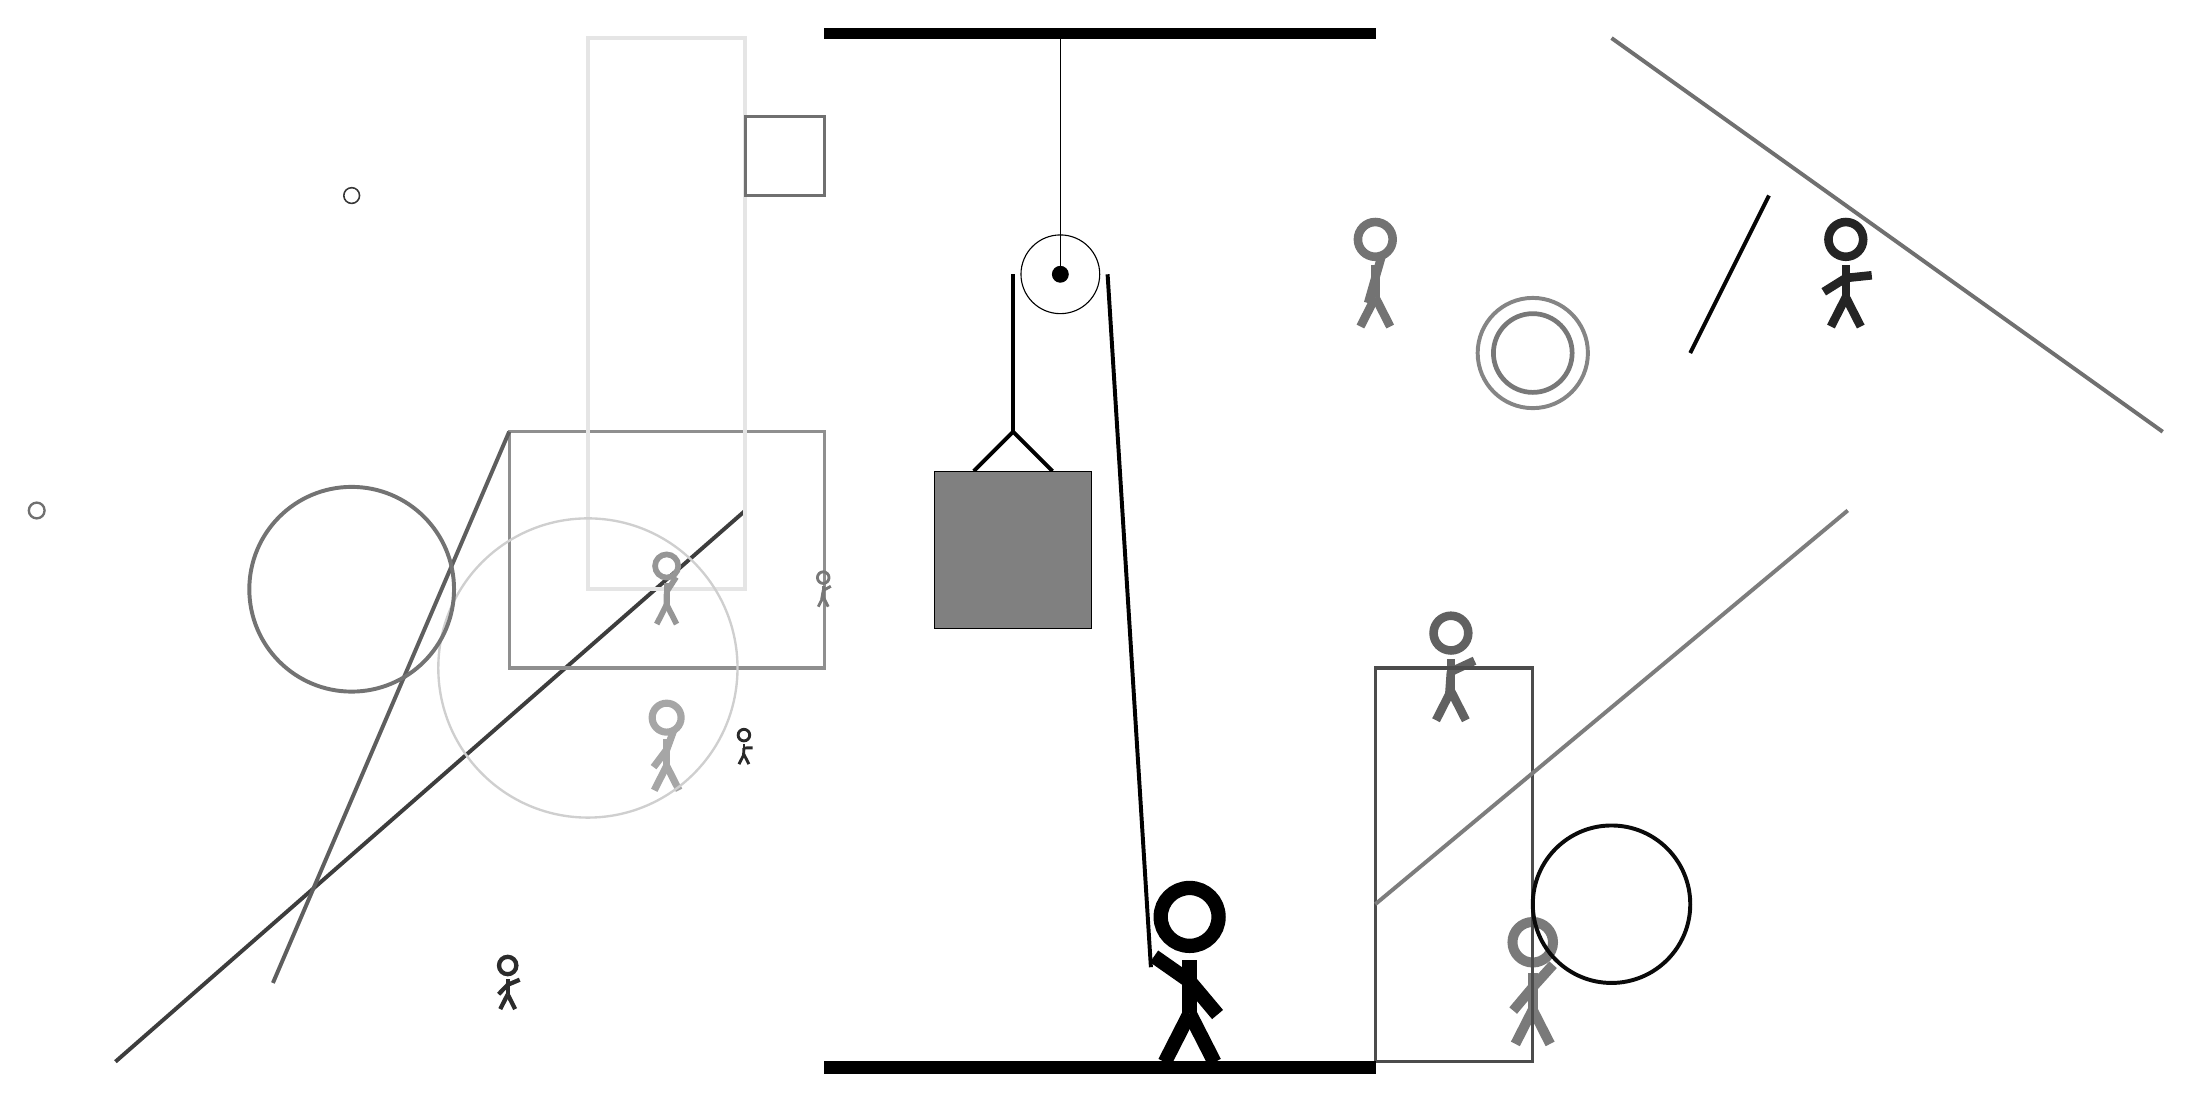
\begin{tikzpicture}
		%%%%% START %%%%%
		
		\draw[fill=black] (-2, 10) rectangle (5, 10.125);
		
		\draw (1, 7) circle (0.5);
		\draw[fill=black] (1, 7) circle (0.1);
		\draw (1, 10) -- (1, 7);
		
		\draw[line width=0.5mm] (-0.1, 4.5) -- (0.4, 5.0) -- (0.9, 4.5);
		\draw[fill=black!50] (-0.6, 4.5) rectangle (1.4, 2.5);
		
		\draw[line width=0.5mm] (0.4, 7) -- (0.4, 5.0);
		\centerarc[line width=0.5mm](1, 7)(0:180:0.6);
		\draw[line width=0.5mm](1.6, 7) -- (2.15, -1.8);
		
		\draw[line width=0.5mm, color=black!56](8, 10) -- (15, 5);
		
		\draw [line width=0.6mm, color=black!53](7, 6) circle (0.5);
		\draw[line width=0.5mm, color=black!76](-3, 4) -- (-11, -3);
		\node[line width=0.2mm, color=black!35] at (-4, 1) {\Strichmaxerl[5][53][70]};
		\node[line width=0.7mm, color=black!52] at (7, -2) {\Strichmaxerl[7][50][48]};
		
		\draw[line width=0.4mm, color=black!44] (-2, 5) rectangle (-6, 2);
		\node[line width=0.6mm, color=black!84] at (-3, 1) {\Strichmaxerl[2][87][1]};
		\node[line width=0.3mm, color=black!62] at (6, 2) {\Strichmaxerl[6][86][25]};
		\draw [line width=0.3mm, color=black!56](-12, 4) circle (0.1);
		
		\draw[line width=0.5mm, color=black!63](-6, 5) -- (-9, -2);
		
		\node[line width=0.6mm, color=black!53] at (-2, 3) {\Strichmaxerl[2][80][29]};
		\draw[line width=0.4mm, color=black!70] (5, -3) rectangle (7, 2);
		\node[line width=0.6mm, color=black!86] at (11, 7) {\Strichmaxerl[6][32][6]};
		\draw [line width=0.5mm, color=black!48](7, 6) circle (0.7);
		\node[line width=0.4mm, color=black!55] at (5, 7) {\Strichmaxerl[6][74][74]};
		\draw[line width=0.5mm, color=black!10] (-3, 3) rectangle (-5, 10);
		\draw[line width=0.5mm, color=black!98](9, 6) -- (10, 8);
		\draw [line width=0.5mm, color=black!96](8, -1) circle (1.0);
		\draw [line width=0.3mm, color=black!19](-5, 2) circle (1.9);
		\draw [line width=0.2mm, color=black!79](-8, 8) circle (0.1);
		\draw[line width=0.4mm, color=black!56] (-3, 9) rectangle (-2, 8);
		\draw[line width=0.5mm, color=black!51](5, -1) -- (11, 4);
		\draw [line width=0.5mm, color=black!55](-8, 3) circle (1.3);
		\node[line width=0.5mm, color=black!41] at (-4, 3) {\Strichmaxerl[4][89][57]};
		\node[line width=0.5mm, color=black!83] at (-6, -2) {\Strichmaxerl[3][46][23]};
		
		
		\node at (2.6, -1.9) {\Strichmaxerl[10][-35][-50]};
		
		\draw[fill=black] (-2, -3) rectangle (5, -3.15);
		
		%%%%% END %%%%%
	\end{tikzpicture}
\end{document}